\chapter{Mask CycleGAN}

\section{Création de la base des données}

\subsection{Les chambres}

Afin de construire une base des données pour la tâche du Image-Painting nous avons amassé des images de chambres aléatoires du web. Ces images contiennent différents motifs et couleurs. 

\begin{figure}[!h]
    \centering
    \subfloat[\centering chambre 1]{{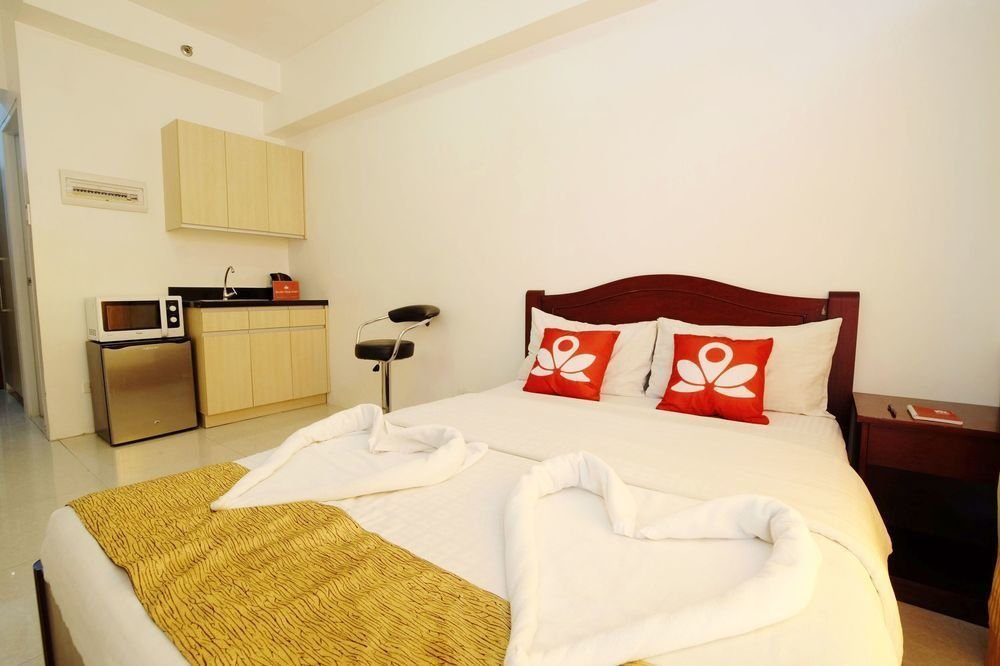
\includegraphics[width=7cm]{images/Mask_CycleGAN/chambre_1.jpg} }}%
    \qquad
    \subfloat[\centering chambre 2]{{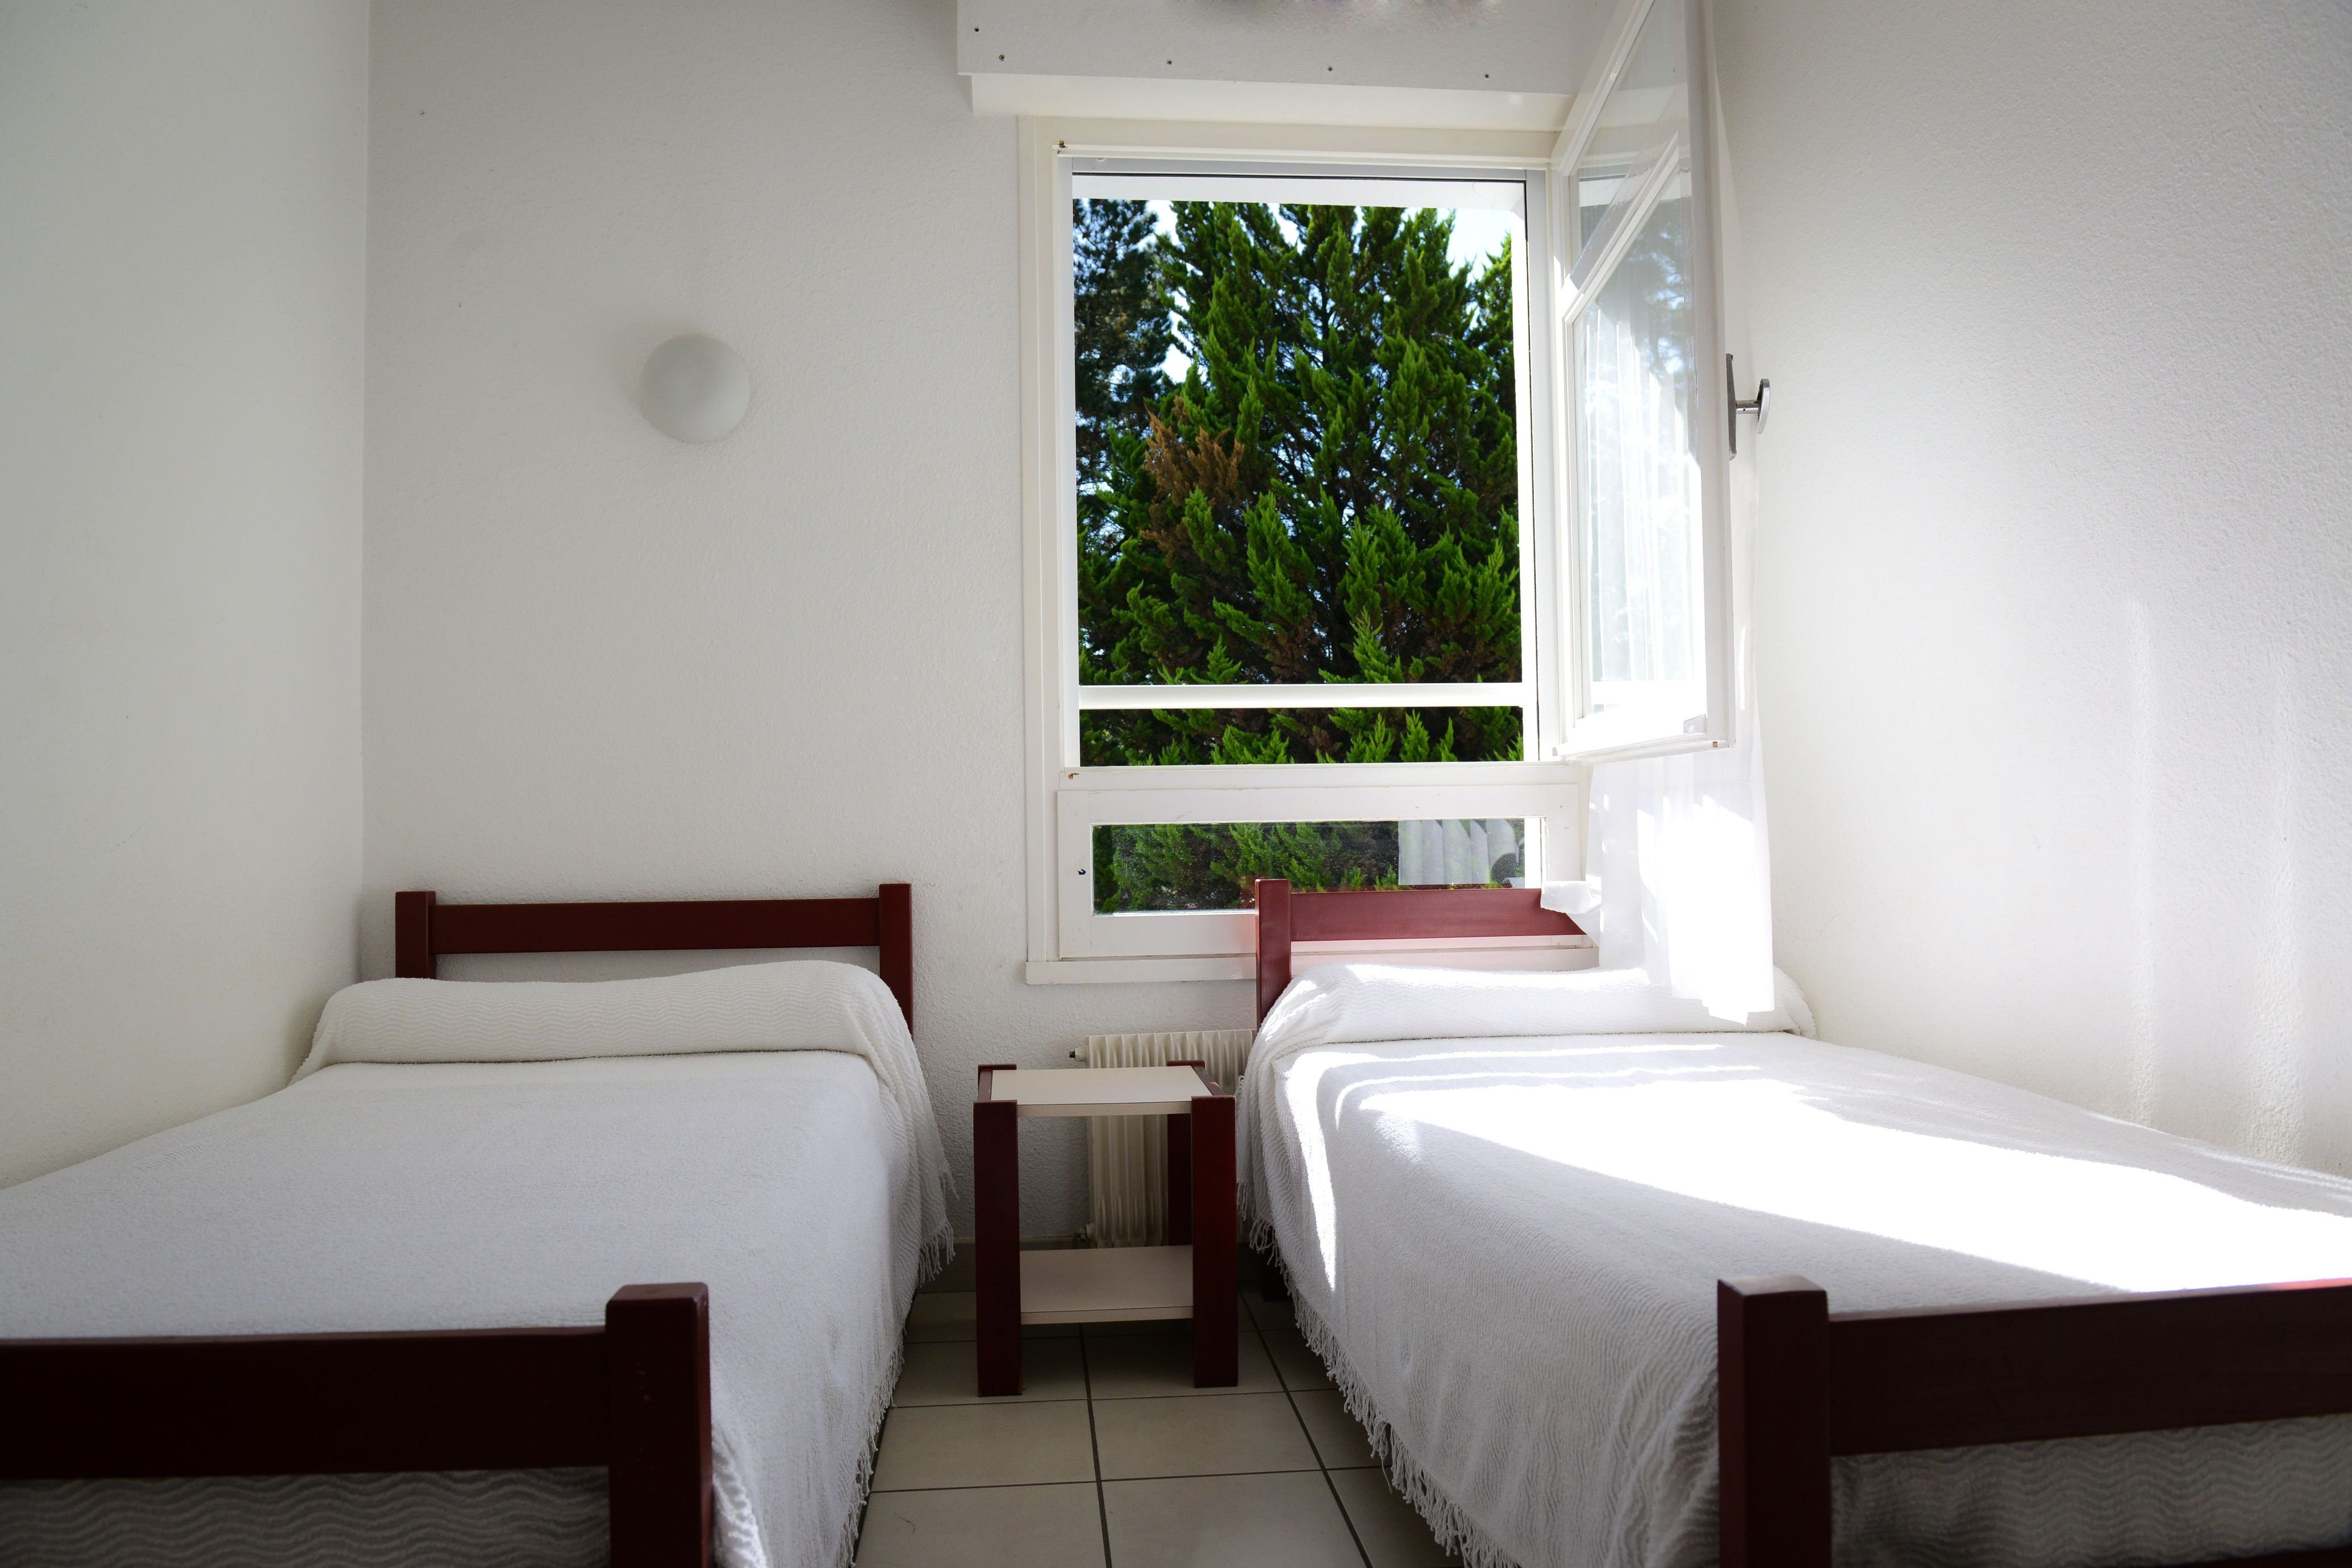
\includegraphics[width=7cm]{images/Mask_CycleGAN/chambre_2.jpg} }}%
    \caption{Exemples d'images trouvées sur le web}%
    \label{fig:example}%
\end{figure}

\subsection{Les masques}
Puis nous avons créé un ensemble de masques détecté/détectable par le Mask-RCNN.

\begin{figure}[!h]
    \centering
    \subfloat[\centering masque 1]{{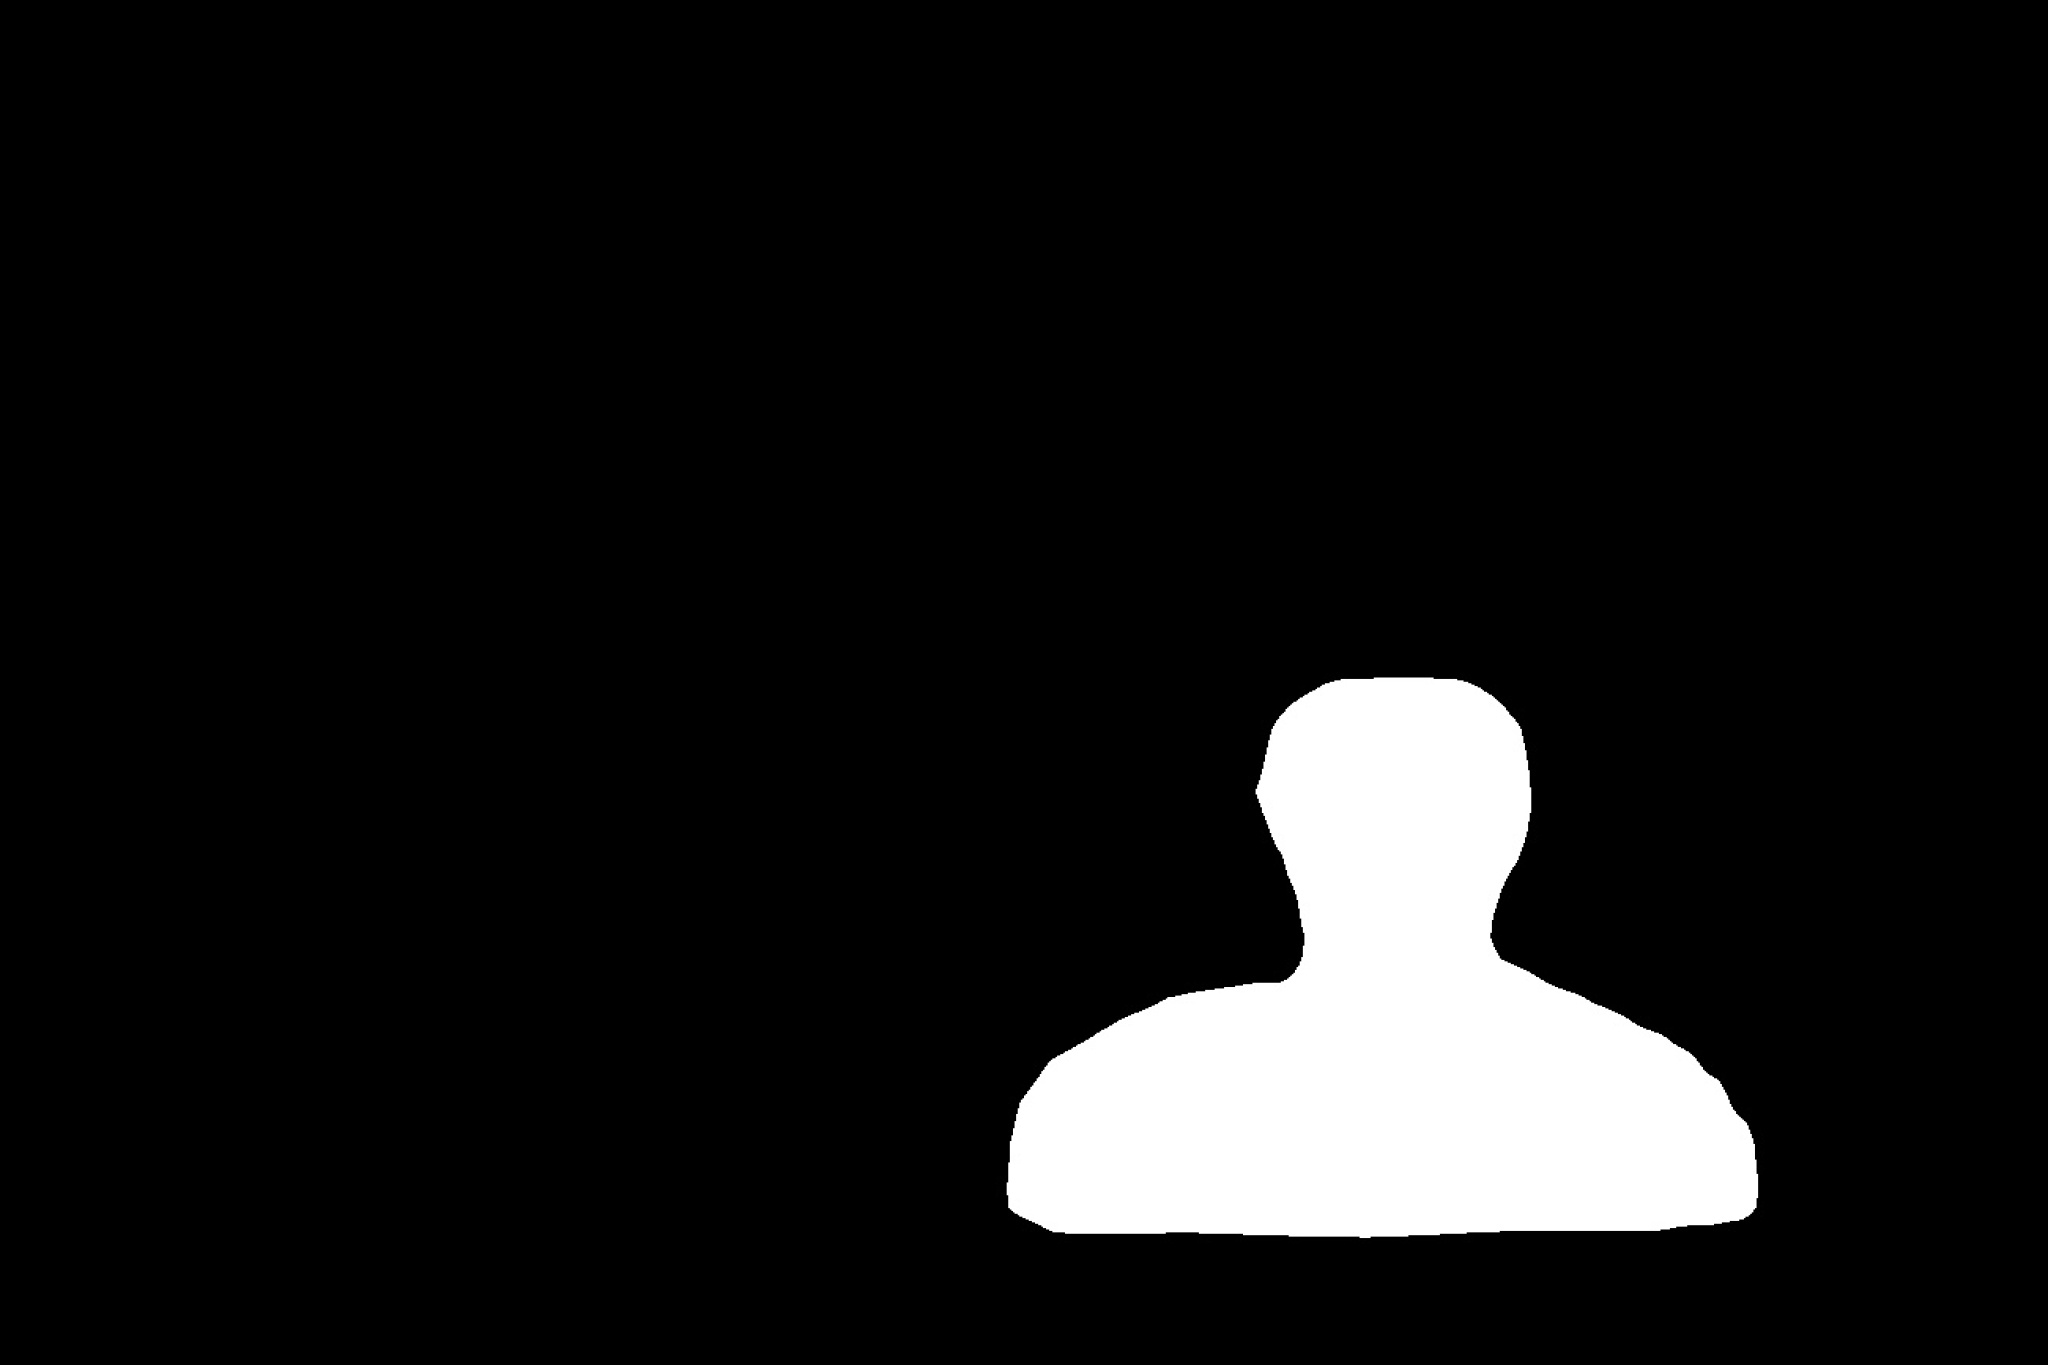
\includegraphics[width=11cm]{images/Mask_CycleGAN/MASK_1.jpg} }}%
    \qquad
    \subfloat[\centering masque 2]{{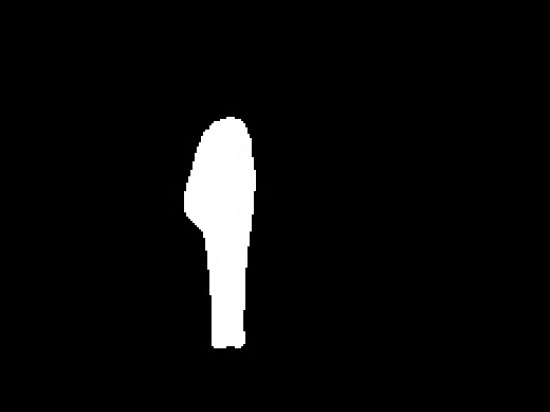
\includegraphics[width=11cm]{images/Mask_CycleGAN/MASK_2.jpg} }}%
    \caption{Exemples de masques générés}%
    \label{fig:example}%
\end{figure}

\subsection{Superposition}
Et finalement, nous avons superposé ces masques avec les images de chamres pour générer une base de données pour l'Image-painting.

\begin{figure}[H]
    \centering
    \subfloat[\centering combinaison 1]{{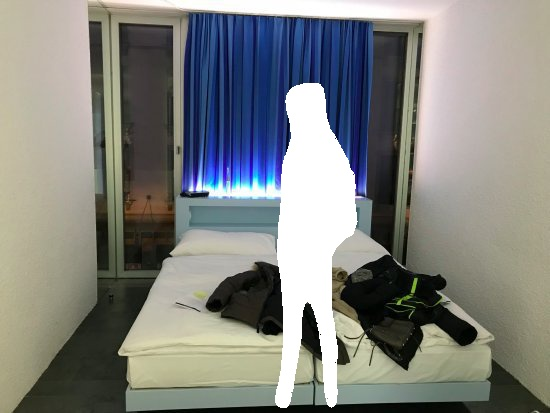
\includegraphics[width=10cm]{images/Mask_CycleGAN/trou_1.jpg} }}%
    \qquad
    \subfloat[\centering combinaison 2]{{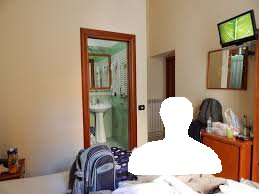
\includegraphics[width=10cm]{images/Mask_CycleGAN/trou_2.jpg} }}%
    \caption{Elements de la base des données}%
    \label{fig:example}%
\end{figure}

\section{Entrainement du CycleGAN}
On lance l'entrainement de l'algorithme avec les même paramètres et hyper-paramètres qu'on a utilisé avant et on obtient les résultats suivants après une centaine d'epochs:

\begin{figure}[H]
    \centering
    \subfloat[\centering remplissage 1]{{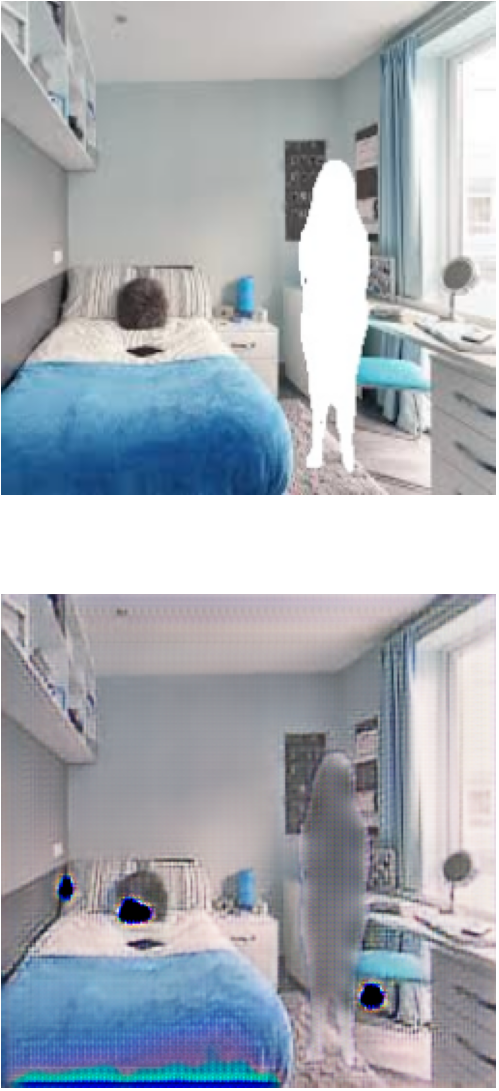
\includegraphics[width=5cm]{images/Mask_CycleGAN/failure_1.png} }}%
    \qquad
    \subfloat[\centering remplissage 2]{{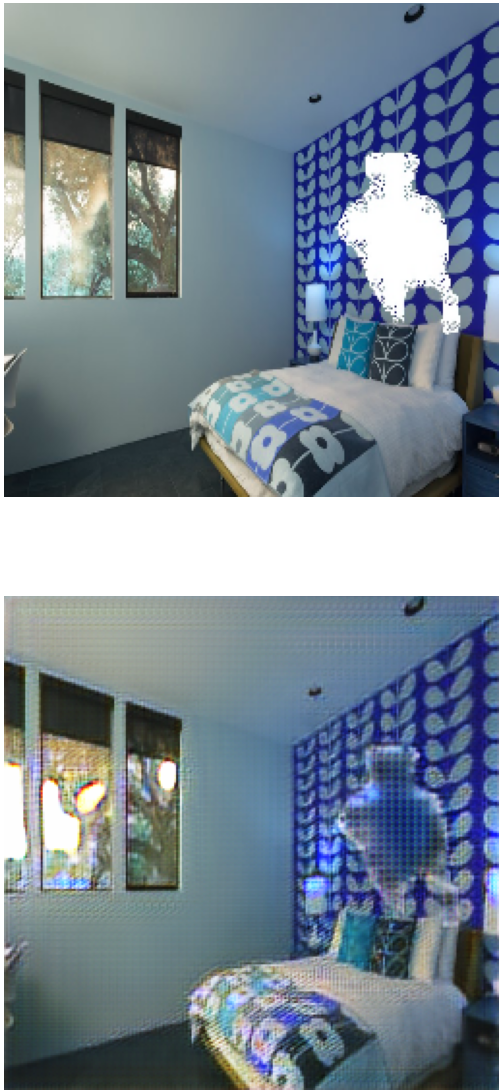
\includegraphics[width=5cm]{images/Mask_CycleGAN/failure_2.png} }}%
    \caption{Elements remplis par le CycleGAN}%
    \label{fig:example}%
\end{figure}

\section{Remarque et observations}
On remarque que l'algorithme a bien compris la tâche qu'il doit effectuer, ce qui n'est pas assez évident parce que une le domaine des images avec une zones blaches (trous) peut se confendre avec le domaine des images en général. Pourtant l CycleGAN a pu localiser le trou et a essayé de trouver un motif ou floutage pour le remplir.
On peut aussi remarquer que l'alorithme a modifié d'autres éléments de l'images et qu'il est confondu par des zones blanches parasites.

\section{Informations non-utilisées}
En effet, même si les images ne sont toujours pas appairées, une nouvelle information peut être extraite des données ; c'est la distinction entre la zone sur lequel l'algrithme doit agir en particulier (la zone blanche créé par le masque) et celle qu'il ne doit pas toucher. On peut donc modifier la fonction de coût pour qu'elle prend en considération cette information pendant l'entrainement.

\section{Nouvelle fonction de coût}
La nouvelle fonction de coût est la même que l'originale mais on lui rajoute un terme qui ressemble au coût du cycle (l'image traversant un cycle de transformation doit être la même) mais pondérée par l'inverse du masque et restrictant la première transformation (demi cycle). Avec la fonction $\mathcal{L}_{\mathrm{demi_cyc}}(G, F)$ de la forme:

$$\mathbb{E}_{b \sim p_{\text {data}}(b)}\left[\|(G(b)-b)\cdot (1 - mask_b)\|_{1}\right]+ \mathbb{E}_{a \sim p_{\text {data}}(a)}\left[\|(F(a)-a)\cdot (1 - mask_b)\|_{1}\right]$$

\section{Résultat final}

Les résultats du derniers entrainement sont encxcore meilleurs:

\begin{figure}[H]
    \centering
    \subfloat[\centering remplissage 1]{{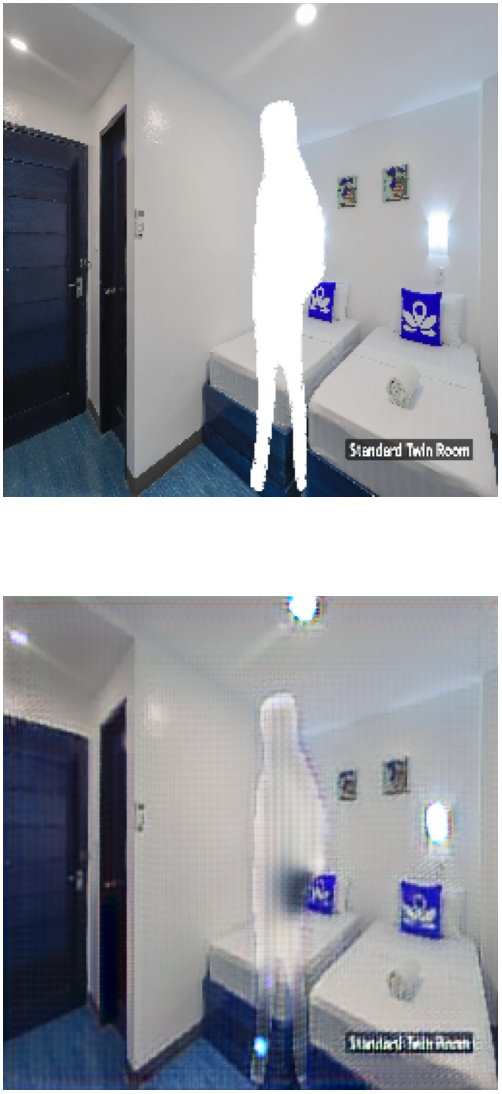
\includegraphics[width=4cm]{images/Mask_CycleGAN/success_1.png} }}%
    \qquad
    \subfloat[\centering remplissage 2]{{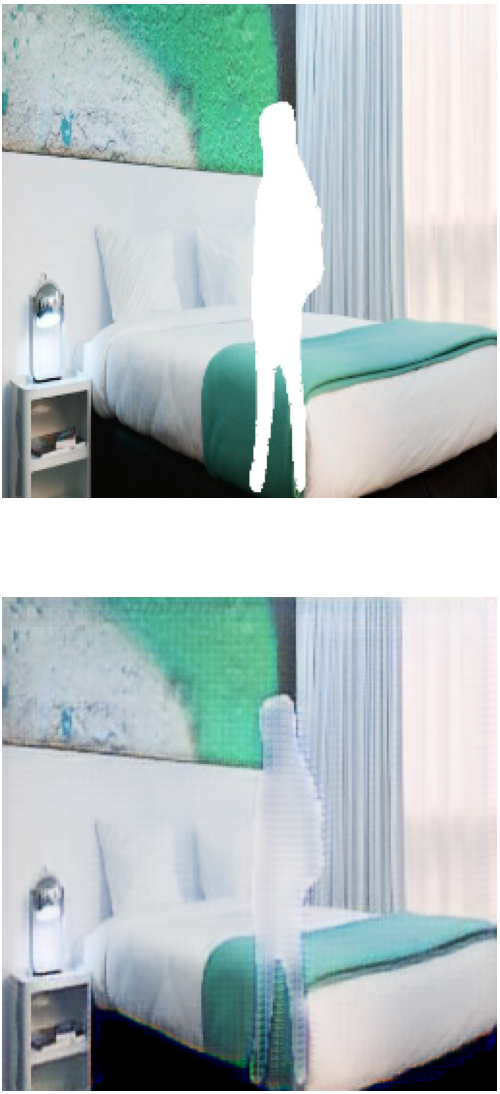
\includegraphics[width=4cm]{images/Mask_CycleGAN/success_2.png} }}%
    \caption{Elements remplis par le CycleGAN modifié}%
    \label{fig:example}%
\end{figure}


